\section{Introduction}
With the recent advances of deep learning, integrating the main modules of automatic speech recognition (ASR) such as acoustic model, pronunciation lexicon and language model into an single end-to-end model is highly attractive. Connectionist Temporal Classification (CTC) \cite{graves2006connectionist} lends itself on such end-to-end approach by introducing an additional blank symbol and specifically-designed loss function optimizing to generate the correct character sequences from the speech signal directly, without framewise phoneme alignment in advance. With many recent results \cite{hannun2014deep, amodei2016deep, collobert2016wav2letter}, end-to-end deep learning has created larger interest in speech community.

However, such end-to-end ASR system requires a huge amount of paired speech-transcription data, which is costly. For most languages in the world, they are lacking of sufficient paired data for training. Pretraining on other language sources as the initialization, then fine-tuning on target language is the dominant approach in such low-resource setting, also known as multilingual transfer learning / pretraining (MultiASR) \cite{vu2014multilingual, tong2017investigation}. The backbone of MultiASR is a multitask model with shared hidden layers (encoder), and many language-specific heads. The idea of such model structure is to learn an encoder to extract language-independent representations to build better acoustic model from many sources of languages. The success of ``language-independent'' features to improve ASR performance compared to monolingual training has been showed in many recent works \cite{cho2018multilingual, dalmia2018sequence}.

\begin{figure}[t]
  \centering
  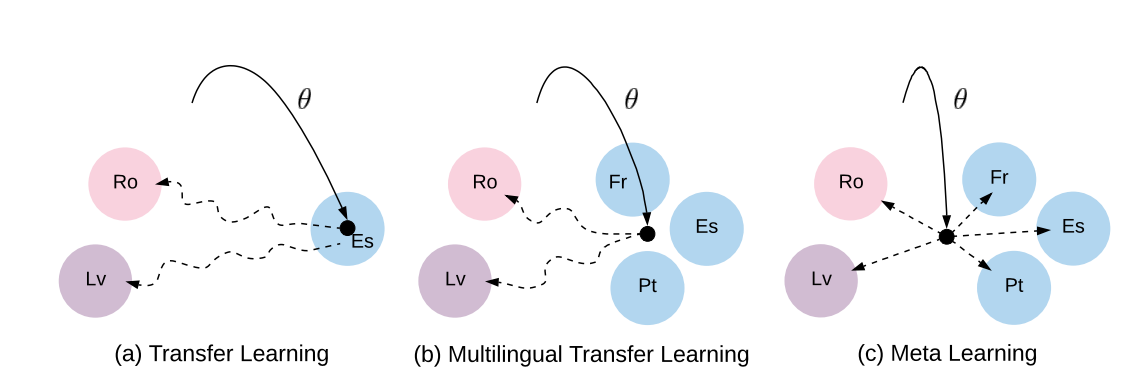
\includegraphics[width=\linewidth]{figs/meta_idea.png}
%  \vspace{2.0cm}
  \label{fig:meta-idea}
  %TODO: Need to be replaced
  \caption{Illustration of the difference between Multitask learning and Meta Learning (\textcolor{red}{WILL BE REPLACED})}

\vspace{-20pt}
\end{figure}

%TODO: sounds weird
With its success, various variants of MultiASR have been proposed. Langauge-adversarial training approaches \cite{Yi2018AdversarialMT, adams2019massively} introduce language-adversarial classification objective to the shared encoder, negating the gradients backproped from the language classifier to encourage the encoder to extract more language-independent representations. Hierarchical approaches \cite{Sanabria2018HierarchicalMT} introduce different granularity objective through combining both character and phoneme prediction at different levels of the model.

In this paper, we provide a novel research direction following up on the idea of multilingual pretraining, \textbf{Meta learning}. Without introducing additional modules like adversarial training, or requiring phoneme level annotation (usually through lexicon) like hierarchical approaches. We only need to modify the optimization process following meta learning training scheme.

Meta learning, or learning-to-learn, has recently received huge interests in machine learning community. The goal of meta learning is to solve the problem of ``fast adaptation on unseen data'', which is aligned with our low-resource setting. With its success in computer vision under few-shot setting \cite{rusu2018meta, snell2017prototypical, vinyals2016matching}, there have been some works in language and speech processing being proposed, for instance, language transfer in neural machine translation \cite{gu2018meta}, dialogue generation \cite{mi2019meta}, and speaker adaptative training \cite{klejch2018learning}.

\textcolor{red}{(TBD BEGIN)} some observation and improvement in our paper \textcolor{red}{(TBD END)}

\label{sec:intro}

